% --------------------------------------------------------------
% This is all preamble stuff that you don't have to worry about.
% Head down to where it says "Start here"
% --------------------------------------------------------------
 
\documentclass[12pt]{article}
\usepackage{graphicx}
\graphicspath{ {images/} }
 
\usepackage[margin=1in]{geometry} 
\usepackage{amsmath,amsthm,amssymb}
\setlength{\parskip}{1em}

\newcommand{\N}{\mathbb{N}}
\newcommand{\Z}{\mathbb{Z}}
 
\newenvironment{theorem}[2][Theorem]{\begin{trivlist}
\item [\hskip \labelsep {\bfseries #1}\hskip \labelsep {\bfseries #2.}]}{\end{trivlist}}
\newenvironment{lemma}[2][Lemma]{\begin{trivlist}
\item [\hskip \labelsep {\bfseries #1}\hskip \labelsep {\bfseries #2.}]}{\end{trivlist}}
\newenvironment{exercise}[2][Exercise]{\begin{trivlist}
\item [\hskip \labelsep {\bfseries #1}\hskip \labelsep {\bfseries #2.}]}{\end{trivlist}}
\newenvironment{problem}[2][Problem]{\begin{trivlist}
\item [\hskip \labelsep {\bfseries #1}\hskip \labelsep {\bfseries #2.}]}{\end{trivlist}}
\newenvironment{question}[2][Question]{\begin{trivlist}
\item [\hskip \labelsep {\bfseries #1}\hskip \labelsep {\bfseries #2.}]}{\end{trivlist}}
\newenvironment{corollary}[2][Corollary]{\begin{trivlist}
\item [\hskip \labelsep {\bfseries #1}\hskip \labelsep {\bfseries #2.}]}{\end{trivlist}}

\newenvironment{solution}{\begin{proof}[Solution]}{\end{proof}}
 
\begin{document}
 
% --------------------------------------------------------------
%                         Start here
% --------------------------------------------------------------
 
\title{Week 7 Writeup}
\author{Arthur Liou}

\maketitle

Prompt: Submitting a write-up of your thoughts, impressions, and any conclusions based on the material from the week. Each week will have its own assignment in the grades page.
\par

\linebreak
For the first part of this week’s writeup, I’m reflecting on the topic – Web Security. MY work lies in SaaS, front and back end web development, so I loved reviewing and learning more about this week’s topic, Web Security. I appreciated working through the lab as part of this week’s topic – straightforward script and very in tune with what we learned right at the end of lecture – the URL classification system.
For what we covered and learned, see my lecture notes below.

\newpage
Lecture Notes: Network Security 
\newline
Lesson 1 – Web Security
\begin{itemize}
\item Web – HTTP/HTML fundamentals 
\item Content, Search Engine, Browsers, WWW, Internet, Networks, Computers
\item 95 of malware is delivered via the web
\item Web Browsing basics. 1.0 &2.0
\item Injection points – de-obfuscated content, Javascript, HTML (DOM Tree), HTML (Raw HTML), HTTP
\item User-level attacks
\item Social Engineering - In the context of information security, refers to psychological manipulation of people into performing actions or divulging confidential information. A type of confidence trick for the purpose of information gathering, fraud, or system access, it differs from a traditional "con" in that it is often one of many steps in a more complex fraud scheme.
\item Phishing, SEO Poisoning, Fake AV, Social Media Link Insertion, Forum Link Insertion, Malvertising
\item A bunch of separate slides for the above 6 topics 
\item User Attack – Common Defenses
\item URL / Domain Reputation Systems, Site Certification Services, Safe URL Shorteners, Client and Gateway AV/AM
\item Browser-level attacks
\item Security features of the modern browser – Content Security Policy Enforcement (Same Origin Policy (SOP), Cross Origin Resource Sharing (CORS), OS Isolation / Sandboxing, and long list of others
\item Browser exploit – downloads, renders and executes, exploits vulnerabilities, typically a multi-step process
\item Content/Script obfuscation
\item Man in the middle attack – intercept and modify traffic in real-time. Requires ability fcor mid-traffic insertion, HTTP
\item Man in the Browser – MITB - Dangerous cousin to the MITM attack - Intercept and modify traffic to/from the server, but INSIDE THE BROWSER
\item DNS Spoofing - AKA “DNS Cache Poisoning”. Phishing, Exploits
\item Clickjacking – UI Redressing – tricks the user into clicking a pre-determined link in a rendered HTML page.
\item Example – Adobe Flash settings
\item SQL injection. BIS, many flavors of SQL injection, not limited to Data
\item Same Origin Policy - Core security feature in all browsers, although not standardized. “Resource from an origin may only access the same origin”
\item Cross-site scripting (XSS) - Goal: Inject client-side script into other user’s browsers. (Bypassing SOP)
\item Cross-site request forgery (XSRF) - The evil brother to XSS, also bypassing SOP
\item Opposite of XSS - Exploit the server’s trust in the browser, not browser’s trust in the server. Goal: Execute malicious actions against a user (as that user!) on their trusted server (i.e. online bank account)
\item Advanced HTML 5 threats – browsers will become more secure
\item HTML5 – Benefits to the Web Designer and User, but also benefits to the malicious actor
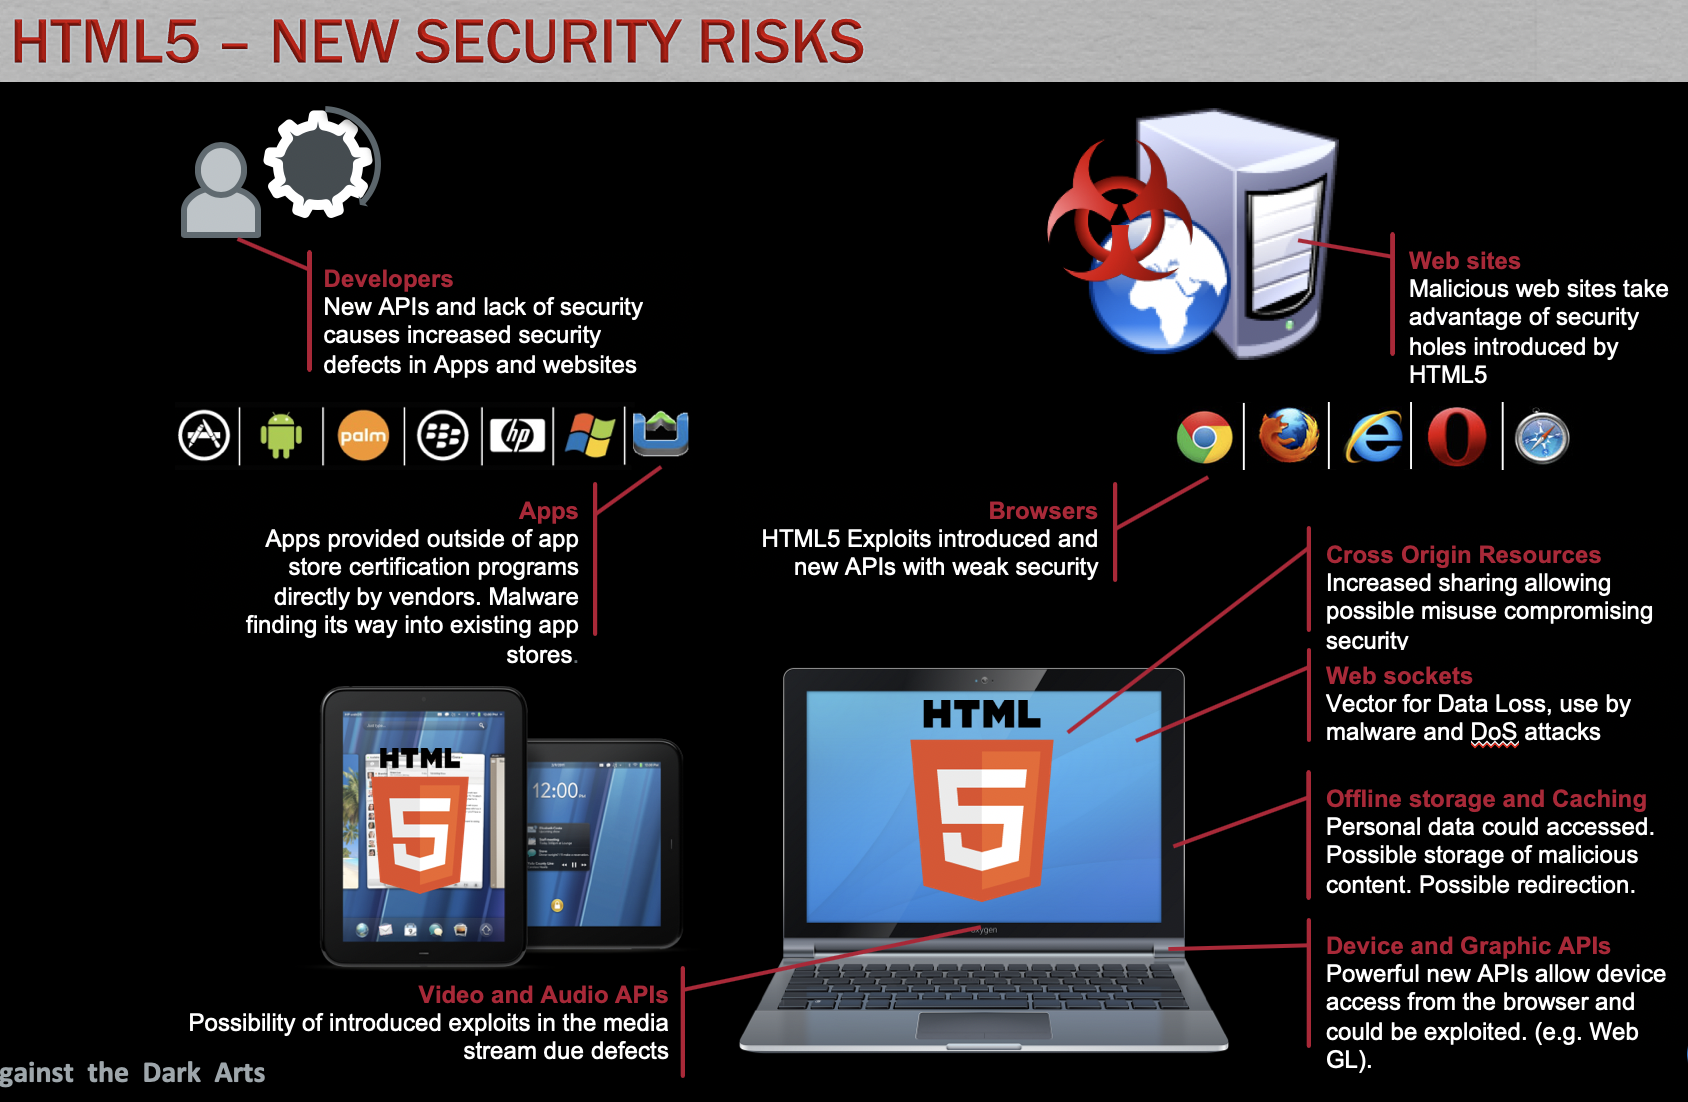
\includegraphics{1.png}
\end{itemize}

Lesson 2
\begin{itemize}
\item Alexa – userful for determining general site popularity and prevalence, data collected via end-user toolbars, domain-based
\item Archiev.org – useful for determining site changes
\item IPVoid – check an IP against a large list of IP blacklists
\item CheckShortUrl – Url Expander service for most short URL services
\item Site Dossier – general site information
\item Webutation – Url reputation clearinghouse
\item Web inspector – online web scanning tool, also list of recently detected malicious sites, classification techniques
\item Virus Total – URL Search, also list of malware files, classification techniques
\item Linux Jwhois, Linux DIG
\item IOC – indicators of compromise – threat feeds, connects the DOTs, provides contextual data around different malicious objects, shareable
\item Research tools
\item PhantomJS – Scripable, headless, webkit browser, executes all scripts and fully renders page, can be driven by many scripting languages, accepts user-defined handlers/callback
\item JSUNPack – detects exploits that target browser and browser plug-in vulnerabilities
\item Burp Suite – intercept and modify traffic to/from the remote site, log resource reqs
\item Webscarab – intercept/modify requests, submission parameter fuzzing, spider
\item Firebug – inexpect HTML elements, explore page script, modify the Dom, breakpoints
\item URL Classification – Manual, Static, Low-interaction, high-interaction
\item How to classify a URL without access to it’s content. Lexical-based, host-based, graph-based
\end{itemize}
% --------------------------------------------------------------
%     You don't have to mess with anything below this line.
% --------------------------------------------------------------
 
\end{document}
